\section{Arithmetic task}

Our ``arithmetic task'' is identical to the ``simple function task'' in the NALU paper \cite{trask-nalu}. However, as they do not describe their dataset generation, dataset parameters, and model evaluation in details we elaborate on that here.

The aim of the ``Arithmetic task'' is to directly test arithmetic models ability to extrapolate beyond the training range. Additionally, our generalized version providing a high degree of flexibility in how the input is shaped, sampled, and the problem complexity.

\begin{figure}[h]
\centering
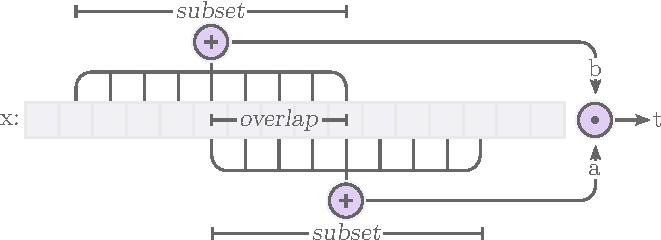
\includegraphics[scale=0.7]{graphics/function_task_static_problem.pdf}
\caption{Shows how the dataset is parameterized.}
\label{fig:simple-function-task-problem}
\end{figure}

\subsection{Dataset generation}
\label{sec:appendix:simple-function-task:data-generation}

The goal is to sum two random subsets of a vector $\mathbf{x}$ ($a$ and $b$), and perform an arithmetic operation on these ($a \circ b$).

\begin{equation}
    a = \sum_{i=s_{1,\mathrm{start}}}^{s_{1,\mathrm{end}}} x_i, \quad b = \sum_{i=s_{2,\mathrm{start}}}^{s_{2,\mathrm{end}}} x_i, \quad t = a \circ b
\end{equation}

Algorithm \ref{alg:simple-function-task-generator} defines the exact procedure to generate the data, where an interpolation range will be used for training and validation and an extrapolation range will be used for testing. Default values are defined in table \ref{tab:simple-function-task-defaults}.

\begin{table}[h]
\caption{Default dataset parameters for ``Arithmetic task''}
\label{tab:simple-function-task-defaults}
\centering
\begin{tabular}{cc}
\begin{minipage}{.4\linewidth}
\begin{tabular}{r l}
\toprule
 Parameter name & Default value \\
 \midrule
 Input size & 100 \\
 Subset ratio & 0.25 \\
 Overlap ratio & 0.5 \\
 \bottomrule
\end{tabular}
\end{minipage} & 
\begin{minipage}{.4\linewidth}
\begin{tabular}{r l}
\toprule
 Parameter name & Default value \\
 \midrule
 Interpolation range & $U[1,2]$ \\
 Extrapolation range & $U[2,6]$ \\
 \\
 \bottomrule
\end{tabular}
\end{minipage}
\end{tabular}
\end{table}

\begin{algorithm}[h]
  \caption{Dataset generation algorithm for ``Arithmetic task''}
  \begin{algorithmic}[1]
    \Function{Dataset}{${\Call{Op}{\cdot, \cdot}: \mathrm{Operation}}$, ${i: \mathrm{Input Size}}$, ${s: \mathrm{Subset Ratio}}$, ${o: \mathrm{Overlap Ratio}}$, ${\hspace{3cm}R: \mathrm{Range}}$}
      \Let{$\mathbf{x}$}{\Call{Uniform}{$R_{lower}, R_{upper}, i$}} \Comment{Sample $i$ elements uniformly}
      \Let{$k$}{\Call{Uniform}{$0, 1 - 2s - o$}} \Comment{Sample offset}
      \Let{$a$}{\Call{Sum}{$\mathbf{x}[ik:i(k+s)]$}} \Comment{Create sum $a$ from subset}
      \Let{$b$}{\Call{Sum}{$\mathbf{x}[i(k+s-o):i (k+2s-0)]$}} \Comment{Create sum $b$ from subset}
      \Let{$t$}{\Call{Op}{$a, b$}} \Comment{Perform operation on $a$ and $b$}
      \State \Return{$x, t$}
    \EndFunction
  \end{algorithmic}
  \label{alg:simple-function-task-generator}
\end{algorithm}

\subsection{Model defintions and setup}

Models are defined in table \ref{tab:simple-function-task-model-defintions} and are all optimized with Adam optimization \cite{adam-optimization} using default parameters, and trained over $5 \cdot 10^6$ iterations. Training takes about 6 hours on a single CPU core(\text{8-Core Intel Xeon E5-2665 2.4GHz}). We run more than 10000 experiments on a HPC cluster.

The training dataset is continuously sampled from the interpolation range where a different seed is used for each experiment, all experiments use a mini-batch size of 128 observations, a fixed validation dataset with $1 \cdot 10^4$ observations sampled from the interpolation range, and a fixed test dataset with $1 \cdot 10^4$ observations sampled from the extrapolation range.

\begin{table}[h]
\caption{Model definitions}
\label{tab:simple-function-task-model-defintions}
\centering
\begin{tabular}{r l l l l l}
\toprule
 Model & Layer 1 & Layer 2 & $\hat{\lambda}_{\mathrm{sparse}}$ & $\lambda_{\mathrm{start}}$ & $\lambda_{\mathrm{end}}$ \\
 \midrule
 NMU & NAU & NMU & 10 & $10^6$ & $2 \cdot 10^6$ \\
 NAU & NAU & NAU & 0.01 & $5 \cdot 10^3$ & $5 \cdot 10^4$ \\
 $\mathrm{NAC}_{\bullet}$ & $\mathrm{NAC}_{+}$ & $\mathrm{NAC}_{\bullet}$ & -- & -- & -- \\
 $\mathrm{NAC}_{\bullet,\sigma}$ & $\mathrm{NAC}_{+}$ & $\mathrm{NAC}_{\bullet,\sigma}$ & -- & -- & -- \\
 $\mathrm{NAC}_{\bullet,\mathrm{NMU}}$ & $\mathrm{NAC}_{+}$ & $\mathrm{NAC}_{\bullet,\mathrm{NMU}}$ & 10 & $10^6$ & $2 \cdot 10^6$ \\
 $\mathrm{NAC}_{+}$ & $\mathrm{NAC}_{+}$ & $\mathrm{NAC}_{+}$ & -- & -- & -- \\
 NALU & NALU & NALU & -- & -- & -- \\
 Linear & Linear & Linear & -- & -- & -- \\
 ReLU & ReLU & ReLU & -- & -- & -- \\
 ReLU6 & ReLU6 & ReLU6 & -- & -- & -- \\
 \bottomrule
\end{tabular}
\end{table}

\subsection{Ablation study}
\label{sec:appendix:ablation-study}
To validate our model, we perform an ablation on the multiplication problem. Some noteworthy observations:

\begin{enumerate}
    \item None of the $W$ constraints, such as $\mathcal{R}_{sparse}$ and clamping W to be in $[0, 1]$, are necessary when the hidden size is just $2$.
    \item Removing the $\mathcal{R}_{sparse}$ causes the NMU to immediately fail for larger hidden sizes.
    \item Removing the clamping of W does not cause much difference. This is because $\mathcal{R}_{sparse}$ also constrains $W$ outside of $[0, 1]$. The regularizer used here is $\mathcal{R}_{sparse} = \min(|W|, |1 - W|)$, which is identical to the one used in other experiments in $[0, 1]$, but is also valid outside $[0, 1]$. Doing this gives only a slightly slower convergence. Although, this can not be guaranteed in general, as the regularizer is omitted during the initial optimization.
    \item Removing both constraints, gives a somewhat satisfying solution, but with a lower success-rate, slower convergence, and higher sparsity error.
\end{enumerate}

In conclusion both constraints are valuable, as they provide faster convergence and a sparser solution, but they are not critical to the success-rate of the NMU.  

\begin{figure}[h]
\centering
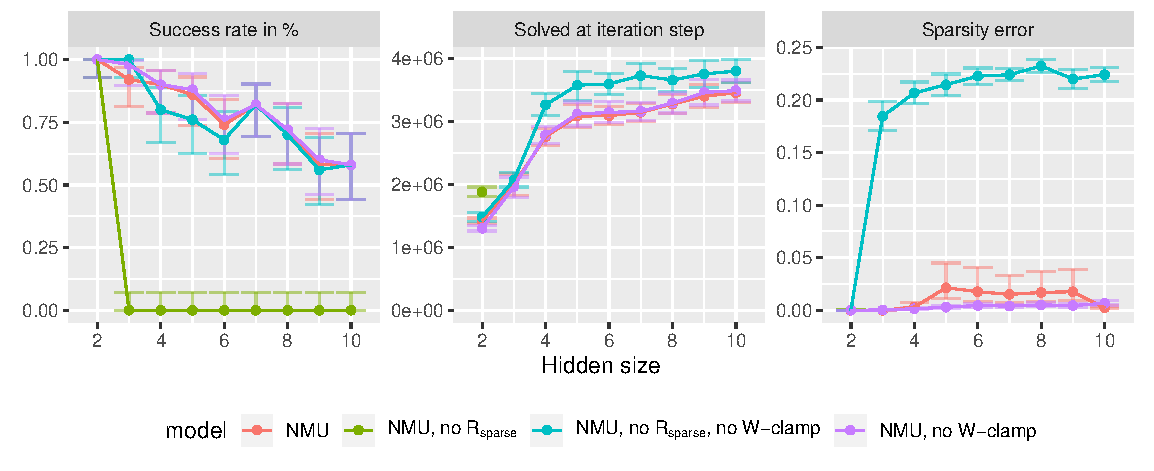
\includegraphics[width=\linewidth]{results/simple_function_static_mul_hidden_size_ablation.pdf}
\caption{Ablation study where $\mathcal{R}_{sparse}$ is removed and the clamping of W is removed. There are 50 experiments with different seeds, for each configuration.}
\label{fig:simple-function-static-ablation}
\end{figure}

\subsection{Effect of dataset parameter}
\label{sec:appendix-simple-function-task:dataset-parameter-effect}

To stress test the models on the multiplication task, we vary the dataset parameters one at a time while keeping the others at their default value (default values in table \ref{tab:simple-function-task-defaults}). Each runs for 50 experiments with different seeds. The results, are visualized in figure \ref{fig:simple-function-static-dataset-parameters-boundary}.

\begin{figure}[h]
\centering
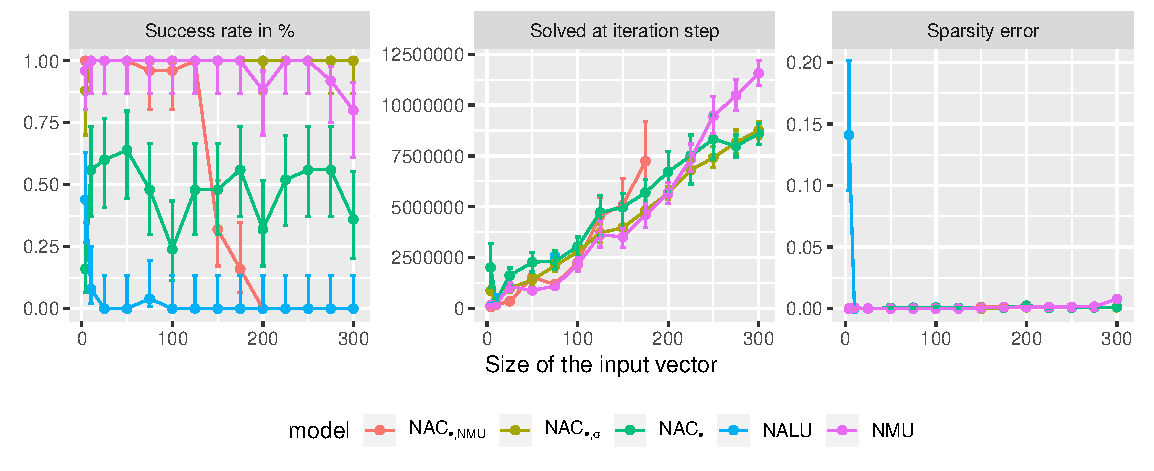
\includegraphics[width=\linewidth,trim={0 1.3cm 0 0},clip]{results/simple_function_static_mul_input_size.pdf}
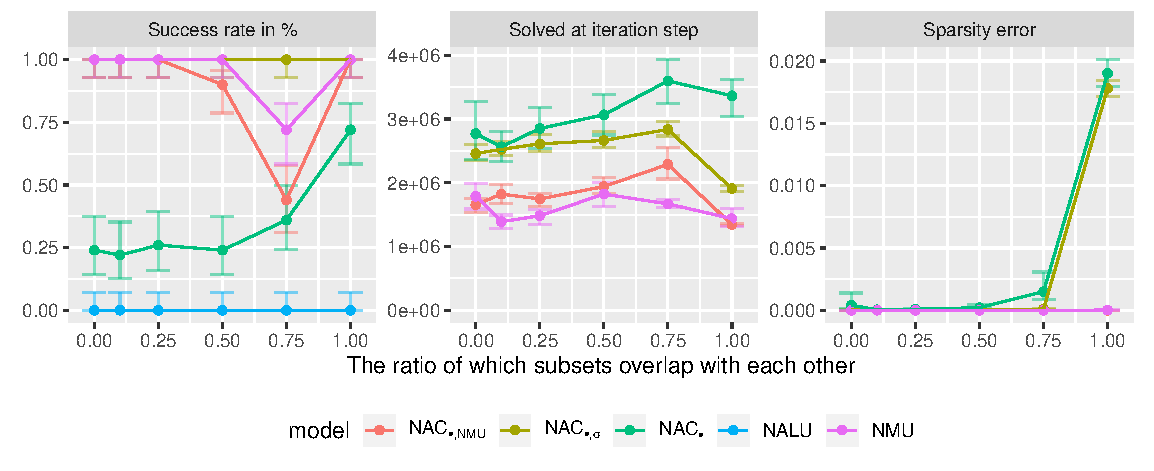
\includegraphics[width=\linewidth,trim={0 1.3cm 0 0.809cm},clip]{results/simple_function_static_mul_overlap.pdf}
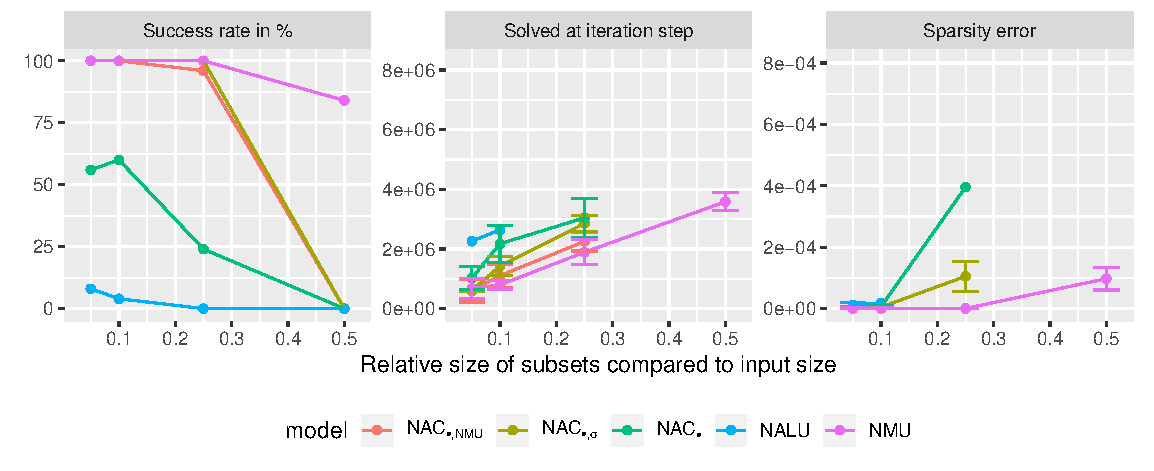
\includegraphics[width=\linewidth,trim={0 0 0 0.809cm},clip]{results/simple_function_static_mul_subset.pdf}
\caption{Shows the effect of the dataset parameters.}
\label{fig:simple-function-static-dataset-parameters-boundary}
\end{figure}

\subsection{NALU gating experiment}
\label{sec:appendix:nalu-gate-experiment}

In the interrest of adding some understand of what goes wrong in the NALU gate, and the shared weight ``hack'' that NALU employees to fix this, we introduce the following experiment.

We train two models, to fit the arithmetic task. Both uses the $\mathrm{NAC}_{+}$ in the first layer and NALU in the second layer. The only difference, is that one model shares the weight between $\mathrm{NAC}_{+}$ and $\mathrm{NAC}_{\bullet}$ in the NALU, and the other just consider them two separate models with separate weights. In both cases NALU should gate between $\mathrm{NAC}_{+}$ and $\mathrm{NAC}_{\bullet}$ and choose the appropriate operation. Note that this NALU model is different from the one presented elsewhere in this paper, including the original NALU paper \cite{trask-nalu}. The typical NALU model, is just two NALU layers with shared weights.

These models are trained for 100 different seeds, on the multiplication and addition task. A histogram of the NALU gate is presented in figure \ref{fig:simple-function-static-nalu-gate-graph} and a summary is presented in table \ref{tab:simple-function-static-nalu-gate-table}. Some noteworthy observations:

\begin{enumerate}
    \item When the weights are separated, far more trials converge to select $\mathrm{NAC}_{+}$, for both the addition and multiplication task.
    \item The performance of the addition task, is strongly correlated with NALU selecting the right operation. In the multiplication task, even if the right gate is selected, $\mathrm{NAC}_{*}$ still struggle to converge consistently, as also seen elsewhere in this paper.
    \item Sharing the weights between $\mathrm{NAC}_{+}$ and $\mathrm{NAC}_{\bullet}$, makes it harder to learn the addition problem. 
\end{enumerate}

These observations validates, that the NALU gate tends to select $\mathrm{NAC}_{+}$, as $\mathrm{NAC}_{+}$ is far easier to learn than $\mathrm{NAC}_{\bullet}$, thus the $\mathrm{NAC}_{+}$ becomes the best estimator early on which the gate will prefer. Once the gate have selected $\mathrm{NAC}_{+}$, it is no longer possible to learn $\mathrm{NAC}_{\bullet}$.

\begin{figure}[h]
\centering
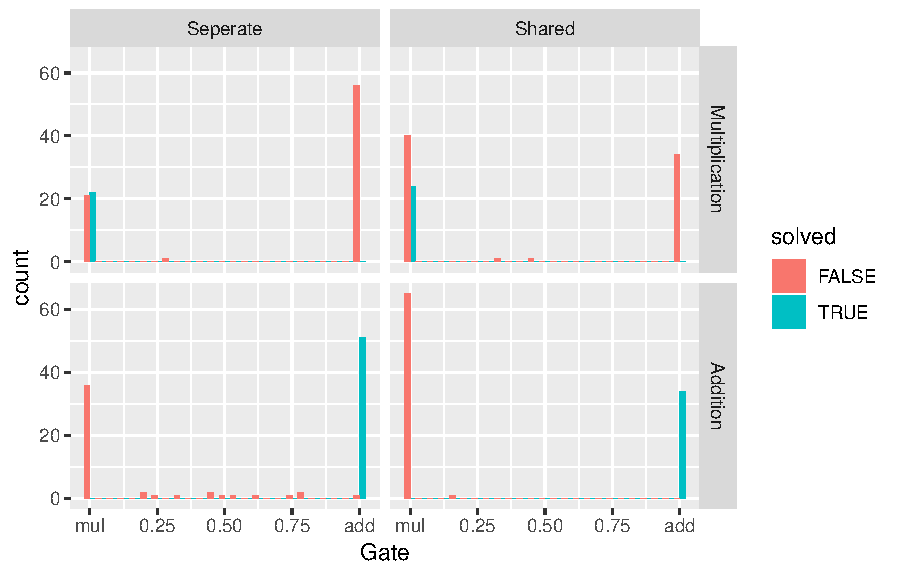
\includegraphics[scale=0.8]{results/function_task_static_nalu.pdf}
\caption{Shows the gating value in the NALU layer followed by a $\mathrm{NAC}_{+}$ layer, where the weights in $\mathrm{NAC}_{+}$ and $\mathrm{NAC}_{\bullet}$ are either shared or separated.}
\label{fig:simple-function-static-nalu-gate-graph}
\end{figure}

\begin{table}[!h]

\caption{\label{tab:simple-function-static-nalu-gate-table}Shows the success-rate, when the model converged, and the sparsity error for all weight matrices, with 95\% confidence interval. Each value is a summary of 100 different seeds.}
\centering
\begin{tabular}{crllll}
\toprule
\multicolumn{1}{c}{Op} & \multicolumn{1}{c}{Model} & \multicolumn{1}{c}{Success} & \multicolumn{2}{c}{Solved at} & \multicolumn{1}{c}{Sparsity error} \\
\cmidrule(l{3pt}r{3pt}){1-1} \cmidrule(l{3pt}r{3pt}){2-2} \cmidrule(l{3pt}r{3pt}){3-3} \cmidrule(l{3pt}r{3pt}){4-5} \cmidrule(l{3pt}r{3pt}){6-6}
 &  & Rate & Median & Mean & Mean\\
\midrule
 & Gated NAU/NMU & $\mathbf{62\%} {~}^{+9\%}_{-10\%}$ & $\mathbf{1.5 \cdot 10^{6}}$ & $\mathbf{1.5 \cdot 10^{6}} {~}^{+3.9 \cdot 10^{4}}_{-3.8 \cdot 10^{4}}$ & $\mathbf{5.0 \cdot 10^{-5}} {~}^{+2.3 \cdot 10^{-5}}_{-1.8 \cdot 10^{-5}}$\\

\nopagebreak
 & NALU (separate) & $22\% {~}^{+9\%}_{-7\%}$ & $2.8 \cdot 10^{6}$ & $3.3 \cdot 10^{6} {~}^{+3.9 \cdot 10^{5}}_{-3.6 \cdot 10^{5}}$ & $5.8 \cdot 10^{-2} {~}^{+4.1 \cdot 10^{-2}}_{-2.3 \cdot 10^{-2}}$\\

\nopagebreak
\multirow{-3}{*}{\centering\arraybackslash $\bm{\times}$} & NALU (shared) & $24\% {~}^{+9\%}_{-7\%}$ & $2.9 \cdot 10^{6}$ & $3.3 \cdot 10^{6} {~}^{+3.7 \cdot 10^{5}}_{-3.6 \cdot 10^{5}}$ & $1.0 \cdot 10^{-3} {~}^{+1.1 \cdot 10^{-3}}_{-4.5 \cdot 10^{-4}}$\\
\cmidrule{1-6}
 & Gated NAU/NMU & $37\% {~}^{+10\%}_{-9\%}$ & $\mathbf{1.9 \cdot 10^{4}}$ & $4.2 \cdot 10^{5} {~}^{+7.3 \cdot 10^{4}}_{-6.7 \cdot 10^{4}}$ & $\mathbf{1.7 \cdot 10^{-1}} {~}^{+4.6 \cdot 10^{-2}}_{-4.0 \cdot 10^{-2}}$\\

\nopagebreak
 & NALU (separate) & $\mathbf{51\%} {~}^{+10\%}_{-10\%}$ & $1.4 \cdot 10^{5}$ & $\mathbf{2.9 \cdot 10^{5}} {~}^{+3.5 \cdot 10^{4}}_{-4.3 \cdot 10^{4}}$ & $1.8 \cdot 10^{-1} {~}^{+1.4 \cdot 10^{-2}}_{-1.4 \cdot 10^{-2}}$\\

\nopagebreak
\multirow{-3}{*}{\centering\arraybackslash $\bm{+}$} & NALU (shared) & $34\% {~}^{+10\%}_{-9\%}$ & $1.8 \cdot 10^{5}$ & $3.1 \cdot 10^{5} {~}^{+4.3 \cdot 10^{4}}_{-5.4 \cdot 10^{4}}$ & $1.8 \cdot 10^{-1} {~}^{+2.3 \cdot 10^{-2}}_{-2.1 \cdot 10^{-2}}$\\
\bottomrule
\end{tabular}
\end{table}


\subsection{Regularization}
\label{sec:appendix:simple-function-task:regualization}

The $\lambda_{start}$ and $\lambda_{end}$ are simply selected based on how much time it takes for the model to converge. The sparsity regularizer should not be used during early optimization, as this part of the optimization is simply about getting each weight on the right side of $\pm 0.5$.

In these experiments the scaling factor $\hat{\lambda}_{\mathrm{sparse}}$ is optimized. 
Results are shown in in figure \ref{fig:simple-fnction-static-regularizer-add}, \ref{fig:simple-fnction-static-regularizer-sub}, and \ref{fig:simple-fnction-static-regularizer-mul}.
\begin{equation}
\lambda_{\mathrm{sparse}} = \hat{\lambda}_{\mathrm{sparse}} \max(\min(\frac{t - \lambda_{\mathrm{start}}}{\lambda_{\mathrm{end}} - \lambda_{\mathrm{start}}}, 1), 0)
\end{equation}

\begin{figure}[H]
\centering
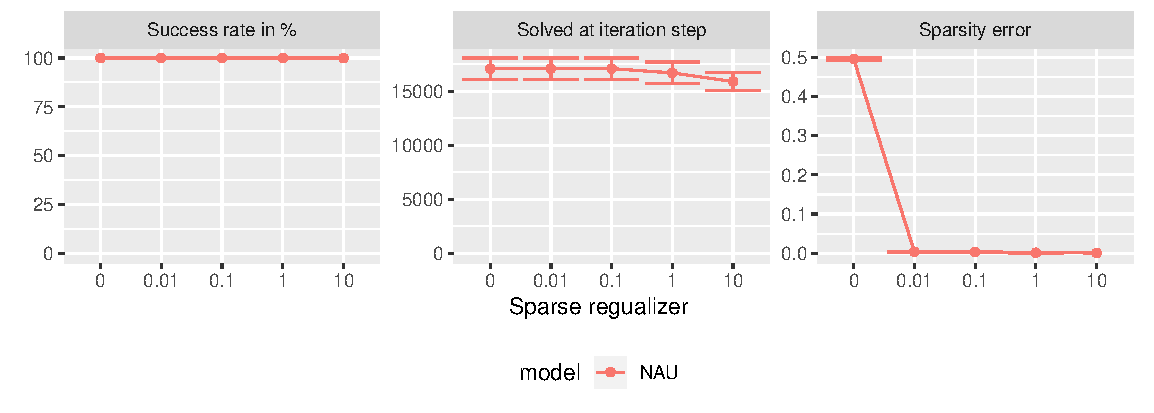
\includegraphics[width=\linewidth]{results/simple_function_static_regualization_add.pdf}
\caption{Shows effect of the scaling factor $\hat{\lambda}_{\mathrm{sparse}}$, on the arithmetic dataset for the $\bm{+}$ operation.}
\label{fig:simple-fnction-static-regularizer-add}
\end{figure}

\begin{figure}[H]
\centering
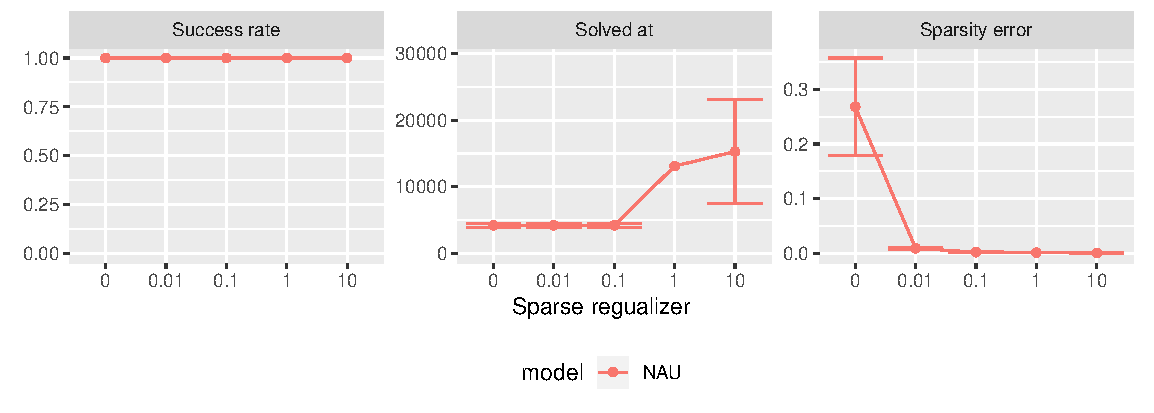
\includegraphics[width=\linewidth]{results/simple_function_static_regualization_sub.pdf}
\caption{Shows effect of the scaling factor $\hat{\lambda}_{\mathrm{sparse}}$, on the arithmetic dataset for the $\bm{-}$ operation.}
\label{fig:simple-fnction-static-regularizer-sub}
\end{figure}

\begin{figure}[H]
\centering
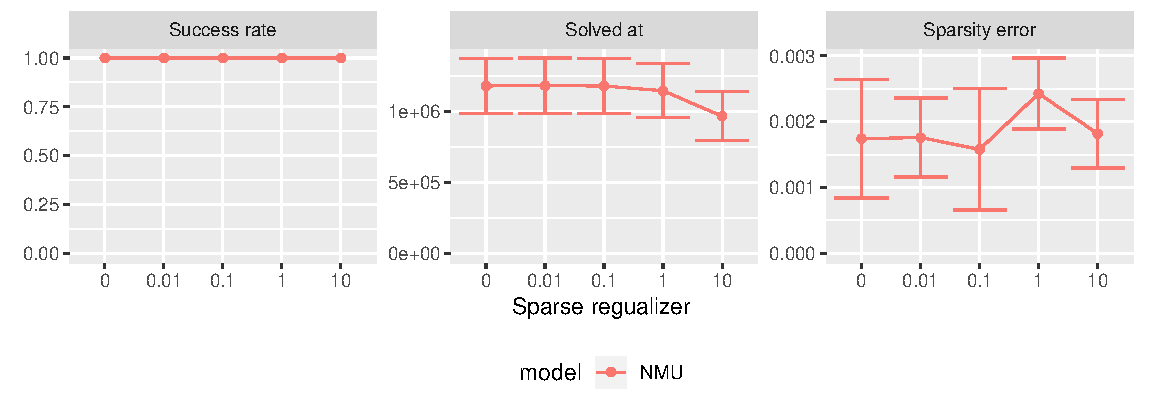
\includegraphics[width=\linewidth]{results/simple_function_static_regualization_mul.pdf}
\caption{Shows effect of the scaling factor $\hat{\lambda}_{\mathrm{sparse}}$, on the arithmetic dataset for the $\bm{\times}$ operation.}
\label{fig:simple-fnction-static-regularizer-mul}
\end{figure}

\subsection{Comparing all models}
\label{sec:appendix:comparison-all-models}

Table \ref{tab:function-task-static-defaults-all} compares all models on all operations used in NALU \cite{trask-nalu}. All variations of model and operation, are trained for 100 different seeds. Some noteworthy observations are:

\begin{enumerate}
    \item Division does not work for any model, including the $NAC_{\bullet}$ and NALU models. This may seam surprising but is actually inline with the results from the NALU paper (\citet{trask-nalu}, table 1), where there is a large error given the interpolation range. The extrapolation range has a smaller error, but this is an artifact of their evaluation method where they normalize with a random baseline. Since a random baseline with have a higher error for the extrapolation range, a similar error will appear to be smaller. If the NALU model had truly learned division to some degree, then both the interpolation and extrapolation range would yield a small error.
    \item $NAC_{\bullet}$ and NALU are barely able to learn $\sqrt{z}$, with just 2\% success-rate for NALU and 7\% success-rate for $NAC_{\bullet}$. Thus we don't belive these models are useful for learning a $\sqrt{z}$ operation.
    \item NMU is fully capable of learning $z^2$. It learns this by learning the subset twice in the NAU layer, this is also how $NAC_{\bullet}$ learns $z^2$.
\end{enumerate}


\begin{longtable}{crllll}
\caption{\label{tab:function-task-static-defaults-all}Shows the success-rate, when the model converged, and the sparsity error for all weight matrices, with 95\% confidence interval. Each value is a summary of 100 different seeds.}\\
\toprule
\multicolumn{1}{c}{Op} & \multicolumn{1}{c}{Model} & \multicolumn{1}{c}{Success} & \multicolumn{2}{c}{Solved at} & \multicolumn{1}{c}{Sparsity error} \\
\cmidrule(l{3pt}r{3pt}){1-1} \cmidrule(l{3pt}r{3pt}){2-2} \cmidrule(l{3pt}r{3pt}){3-3} \cmidrule(l{3pt}r{3pt}){4-5} \cmidrule(l{3pt}r{3pt}){6-6}
 &  & Rate & Median & Mean & Mean\\
\midrule
\endfirsthead
\caption[]{Shows the success-rate, when the model converged, and the sparsity error for all weight matrices, with 95\% confidence interval. Each value is a summary of 100 different seeds. \textit{(continued)}}\\
\toprule
\multicolumn{1}{c}{Op} & \multicolumn{1}{c}{Model} & \multicolumn{1}{c}{Success} & \multicolumn{2}{c}{Solved at} & \multicolumn{1}{c}{Sparsity error} \\
\cmidrule(l{3pt}r{3pt}){1-1} \cmidrule(l{3pt}r{3pt}){2-2} \cmidrule(l{3pt}r{3pt}){3-3} \cmidrule(l{3pt}r{3pt}){4-5} \cmidrule(l{3pt}r{3pt}){6-6}
 &  & Rate & Median & Mean & Mean\\
\midrule
\endhead
\
\endfoot
\bottomrule
\endlastfoot
 & $\mathrm{NAC}_{\bullet,\mathrm{NMU}}$ & $93\% {~}^{+4\%}_{-7\%}$ & $1.8 \cdot 10^{6}$ & $1.9 \cdot 10^{6} {~}^{+7.7 \cdot 10^{4}}_{-9.3 \cdot 10^{4}}$ & $9.5 \cdot 10^{-7} {~}^{+4.2 \cdot 10^{-7}}_{-4.2 \cdot 10^{-7}}$\\

\nopagebreak
 & $\mathrm{NAC}_{\bullet,\sigma}$ & $\mathbf{100\%} {~}^{+0\%}_{-4\%}$ & $2.5 \cdot 10^{6}$ & $2.6 \cdot 10^{6} {~}^{+8.8 \cdot 10^{4}}_{-7.2 \cdot 10^{4}}$ & $4.6 \cdot 10^{-5} {~}^{+5.0 \cdot 10^{-6}}_{-5.6 \cdot 10^{-6}}$\\

\nopagebreak
 & $\mathrm{NAC}_{\bullet}$ & $31\% {~}^{+10\%}_{-8\%}$ & $2.8 \cdot 10^{6}$ & $3.0 \cdot 10^{6} {~}^{+2.9 \cdot 10^{5}}_{-2.4 \cdot 10^{5}}$ & $5.8 \cdot 10^{-4} {~}^{+4.8 \cdot 10^{-4}}_{-2.6 \cdot 10^{-4}}$\\

\nopagebreak
 & $\mathrm{NAC}_{+}$ & $0\% {~}^{+4\%}_{-0\%}$ & --- & --- & ---\\

\nopagebreak
 & Linear & $0\% {~}^{+4\%}_{-0\%}$ & --- & --- & ---\\

\nopagebreak
 & NALU & $0\% {~}^{+4\%}_{-0\%}$ & --- & --- & ---\\

\nopagebreak
 & NAU & $0\% {~}^{+4\%}_{-0\%}$ & --- & --- & ---\\

\nopagebreak
 & NMU & $98\% {~}^{+1\%}_{-5\%}$ & $\mathbf{1.4 \cdot 10^{6}}$ & $\mathbf{1.5 \cdot 10^{6}} {~}^{+4.8 \cdot 10^{4}}_{-6.5 \cdot 10^{4}}$ & $\mathbf{4.2 \cdot 10^{-7}} {~}^{+2.9 \cdot 10^{-8}}_{-2.9 \cdot 10^{-8}}$\\

\nopagebreak
 & ReLU & $0\% {~}^{+4\%}_{-0\%}$ & --- & --- & ---\\

\nopagebreak
\multirow{-10}{*}{\centering\arraybackslash $\bm{\times}$} & ReLU6 & $0\% {~}^{+4\%}_{-0\%}$ & --- & --- & ---\\
\cmidrule{1-6}
 & $\mathrm{NAC}_{\bullet,\mathrm{NMU}}$ & $\mathbf{0\%} {~}^{+4\%}_{-0\%}$ & --- & --- & ---\\

\nopagebreak
 & $\mathrm{NAC}_{\bullet,\sigma}$ & $\mathbf{0\%} {~}^{+4\%}_{-0\%}$ & --- & --- & ---\\

\nopagebreak
 & $\mathrm{NAC}_{\bullet}$ & $\mathbf{0\%} {~}^{+4\%}_{-0\%}$ & --- & --- & ---\\

\nopagebreak
 & $\mathrm{NAC}_{+}$ & $\mathbf{0\%} {~}^{+4\%}_{-0\%}$ & --- & --- & ---\\

\nopagebreak
 & Linear & $\mathbf{0\%} {~}^{+4\%}_{-0\%}$ & --- & --- & ---\\

\nopagebreak
 & NALU & $\mathbf{0\%} {~}^{+4\%}_{-0\%}$ & --- & --- & ---\\

\nopagebreak
 & NAU & $\mathbf{0\%} {~}^{+4\%}_{-0\%}$ & --- & --- & ---\\

\nopagebreak
 & NMU & $\mathbf{0\%} {~}^{+4\%}_{-0\%}$ & --- & --- & ---\\

\nopagebreak
 & ReLU & $\mathbf{0\%} {~}^{+4\%}_{-0\%}$ & --- & --- & ---\\

\nopagebreak
\multirow{-10}{*}{\centering\arraybackslash $\bm{\mathbin{/}}$} & ReLU6 & $\mathbf{0\%} {~}^{+4\%}_{-0\%}$ & --- & --- & ---\\
\cmidrule{1-6}
 & $\mathrm{NAC}_{\bullet,\mathrm{NMU}}$ & $0\% {~}^{+4\%}_{-0\%}$ & --- & --- & ---\\

\nopagebreak
 & $\mathrm{NAC}_{\bullet,\sigma}$ & $0\% {~}^{+4\%}_{-0\%}$ & --- & --- & ---\\

\nopagebreak
 & $\mathrm{NAC}_{\bullet}$ & $0\% {~}^{+4\%}_{-0\%}$ & --- & --- & ---\\

\nopagebreak
 & $\mathrm{NAC}_{+}$ & $\mathbf{100\%} {~}^{+0\%}_{-4\%}$ & $2.5 \cdot 10^{5}$ & $4.9 \cdot 10^{5} {~}^{+5.2 \cdot 10^{4}}_{-4.5 \cdot 10^{4}}$ & $2.3 \cdot 10^{-1} {~}^{+6.5 \cdot 10^{-3}}_{-6.5 \cdot 10^{-3}}$\\

\nopagebreak
 & Linear & $\mathbf{100\%} {~}^{+0\%}_{-4\%}$ & $6.1 \cdot 10^{4}$ & $\mathbf{6.3 \cdot 10^{4}} {~}^{+2.5 \cdot 10^{3}}_{-3.3 \cdot 10^{3}}$ & $2.5 \cdot 10^{-1} {~}^{+3.6 \cdot 10^{-4}}_{-3.6 \cdot 10^{-4}}$\\

\nopagebreak
 & NALU & $14\% {~}^{+8\%}_{-5\%}$ & $1.5 \cdot 10^{6}$ & $1.6 \cdot 10^{6} {~}^{+3.8 \cdot 10^{5}}_{-3.3 \cdot 10^{5}}$ & $1.7 \cdot 10^{-1} {~}^{+2.7 \cdot 10^{-2}}_{-2.5 \cdot 10^{-2}}$\\

\nopagebreak
 & NAU & $\mathbf{100\%} {~}^{+0\%}_{-4\%}$ & $\mathbf{1.8 \cdot 10^{4}}$ & $3.9 \cdot 10^{5} {~}^{+4.4 \cdot 10^{4}}_{-3.7 \cdot 10^{4}}$ & $\mathbf{3.2 \cdot 10^{-5}} {~}^{+1.3 \cdot 10^{-5}}_{-1.3 \cdot 10^{-5}}$\\

\nopagebreak
 & NMU & $0\% {~}^{+4\%}_{-0\%}$ & --- & --- & ---\\

\nopagebreak
 & ReLU & $62\% {~}^{+9\%}_{-10\%}$ & $6.2 \cdot 10^{4}$ & $7.6 \cdot 10^{4} {~}^{+8.3 \cdot 10^{3}}_{-7.0 \cdot 10^{3}}$ & $2.5 \cdot 10^{-1} {~}^{+2.4 \cdot 10^{-3}}_{-2.4 \cdot 10^{-3}}$\\

\nopagebreak
\multirow{-10}{*}{\centering\arraybackslash $\bm{+}$} & ReLU6 & $0\% {~}^{+4\%}_{-0\%}$ & --- & --- & ---\\
\cmidrule{1-6}
 & $\mathrm{NAC}_{\bullet,\mathrm{NMU}}$ & $0\% {~}^{+4\%}_{-0\%}$ & --- & --- & ---\\

\nopagebreak
 & $\mathrm{NAC}_{\bullet,\sigma}$ & $0\% {~}^{+4\%}_{-0\%}$ & --- & --- & ---\\

\nopagebreak
 & $\mathrm{NAC}_{\bullet}$ & $0\% {~}^{+4\%}_{-0\%}$ & --- & --- & ---\\

\nopagebreak
 & $\mathrm{NAC}_{+}$ & $\mathbf{100\%} {~}^{+0\%}_{-4\%}$ & $9.0 \cdot 10^{3}$ & $3.7 \cdot 10^{5} {~}^{+3.8 \cdot 10^{4}}_{-3.8 \cdot 10^{4}}$ & $2.3 \cdot 10^{-1} {~}^{+5.4 \cdot 10^{-3}}_{-5.4 \cdot 10^{-3}}$\\

\nopagebreak
 & Linear & $7\% {~}^{+7\%}_{-4\%}$ & $3.3 \cdot 10^{6}$ & $1.4 \cdot 10^{6} {~}^{+7.0 \cdot 10^{5}}_{-6.1 \cdot 10^{5}}$ & $1.8 \cdot 10^{-1} {~}^{+7.2 \cdot 10^{-2}}_{-5.8 \cdot 10^{-2}}$\\

\nopagebreak
 & NALU & $14\% {~}^{+8\%}_{-5\%}$ & $1.9 \cdot 10^{6}$ & $1.9 \cdot 10^{6} {~}^{+4.4 \cdot 10^{5}}_{-4.5 \cdot 10^{5}}$ & $2.1 \cdot 10^{-1} {~}^{+2.2 \cdot 10^{-2}}_{-2.2 \cdot 10^{-2}}$\\

\nopagebreak
 & NAU & $\mathbf{100\%} {~}^{+0\%}_{-4\%}$ & $\mathbf{5.0 \cdot 10^{3}}$ & $\mathbf{1.6 \cdot 10^{5}} {~}^{+1.7 \cdot 10^{4}}_{-1.6 \cdot 10^{4}}$ & $6.6 \cdot 10^{-2} {~}^{+2.5 \cdot 10^{-2}}_{-1.9 \cdot 10^{-2}}$\\

\nopagebreak
 & NMU & $56\% {~}^{+9\%}_{-10\%}$ & $1.0 \cdot 10^{6}$ & $1.0 \cdot 10^{6} {~}^{+5.8 \cdot 10^{2}}_{-5.8 \cdot 10^{2}}$ & $\mathbf{3.4 \cdot 10^{-4}} {~}^{+3.2 \cdot 10^{-5}}_{-2.6 \cdot 10^{-5}}$\\

\nopagebreak
 & ReLU & $0\% {~}^{+4\%}_{-0\%}$ & --- & --- & ---\\

\nopagebreak
\multirow{-10}{*}{\centering\arraybackslash $\bm{-}$} & ReLU6 & $0\% {~}^{+4\%}_{-0\%}$ & --- & --- & ---\\
\cmidrule{1-6}
 & $\mathrm{NAC}_{\bullet,\mathrm{NMU}}$ & $3\% {~}^{+5\%}_{-2\%}$ & $1.0 \cdot 10^{6}$ & $\mathbf{1.0 \cdot 10^{6}}$ & $\mathbf{1.7 \cdot 10^{-1}} {~}^{+8.3 \cdot 10^{-3}}_{-8.1 \cdot 10^{-3}}$\\

\nopagebreak
 & $\mathrm{NAC}_{\bullet,\sigma}$ & $0\% {~}^{+4\%}_{-0\%}$ & --- & --- & ---\\

\nopagebreak
 & $\mathrm{NAC}_{\bullet}$ & $\mathbf{7\%} {~}^{+7\%}_{-4\%}$ & $\mathbf{4.0 \cdot 10^{5}}$ & $1.5 \cdot 10^{6} {~}^{+6.0 \cdot 10^{5}}_{-5.6 \cdot 10^{5}}$ & $2.4 \cdot 10^{-1} {~}^{+1.7 \cdot 10^{-2}}_{-1.7 \cdot 10^{-2}}$\\

\nopagebreak
 & $\mathrm{NAC}_{+}$ & $0\% {~}^{+4\%}_{-0\%}$ & --- & --- & ---\\

\nopagebreak
 & Linear & $0\% {~}^{+4\%}_{-0\%}$ & --- & --- & ---\\

\nopagebreak
 & NALU & $2\% {~}^{+5\%}_{-1\%}$ & $2.6 \cdot 10^{6}$ & $3.3 \cdot 10^{6} {~}^{+1.8 \cdot 10^{6}}_{-2.2 \cdot 10^{6}}$ & $5.0 \cdot 10^{-1} {~}^{+2.5 \cdot 10^{-6}}_{-8.0 \cdot 10^{-6}}$\\

\nopagebreak
 & NAU & $0\% {~}^{+4\%}_{-0\%}$ & --- & --- & ---\\

\nopagebreak
 & NMU & $0\% {~}^{+4\%}_{-0\%}$ & --- & --- & ---\\

\nopagebreak
 & ReLU & $0\% {~}^{+4\%}_{-0\%}$ & --- & --- & ---\\

\nopagebreak
\multirow{-10}{*}{\centering\arraybackslash $\sqrt{z}$} & ReLU6 & $0\% {~}^{+4\%}_{-0\%}$ & --- & --- & ---\\
\cmidrule{1-6}
 & $\mathrm{NAC}_{\bullet,\mathrm{NMU}}$ & $\mathbf{100\%} {~}^{+0\%}_{-4\%}$ & $1.4 \cdot 10^{6}$ & $1.5 \cdot 10^{6} {~}^{+7.1 \cdot 10^{4}}_{-5.9 \cdot 10^{4}}$ & $\mathbf{2.9 \cdot 10^{-7}} {~}^{+1.4 \cdot 10^{-8}}_{-1.4 \cdot 10^{-8}}$\\

\nopagebreak
 & $\mathrm{NAC}_{\bullet,\sigma}$ & $\mathbf{100\%} {~}^{+0\%}_{-4\%}$ & $1.9 \cdot 10^{6}$ & $1.9 \cdot 10^{6} {~}^{+5.3 \cdot 10^{4}}_{-6.2 \cdot 10^{4}}$ & $1.8 \cdot 10^{-2} {~}^{+4.3 \cdot 10^{-4}}_{-4.3 \cdot 10^{-4}}$\\

\nopagebreak
 & $\mathrm{NAC}_{\bullet}$ & $77\% {~}^{+7\%}_{-9\%}$ & $3.3 \cdot 10^{6}$ & $3.2 \cdot 10^{6} {~}^{+1.6 \cdot 10^{5}}_{-2.0 \cdot 10^{5}}$ & $1.8 \cdot 10^{-2} {~}^{+5.8 \cdot 10^{-4}}_{-5.7 \cdot 10^{-4}}$\\

\nopagebreak
 & $\mathrm{NAC}_{+}$ & $0\% {~}^{+4\%}_{-0\%}$ & --- & --- & ---\\

\nopagebreak
 & Linear & $0\% {~}^{+4\%}_{-0\%}$ & --- & --- & ---\\

\nopagebreak
 & NALU & $0\% {~}^{+4\%}_{-0\%}$ & --- & --- & ---\\

\nopagebreak
 & NAU & $0\% {~}^{+4\%}_{-0\%}$ & --- & --- & ---\\

\nopagebreak
 & NMU & $\mathbf{100\%} {~}^{+0\%}_{-4\%}$ & $\mathbf{1.2 \cdot 10^{6}}$ & $\mathbf{1.3 \cdot 10^{6}} {~}^{+3.1 \cdot 10^{4}}_{-3.6 \cdot 10^{4}}$ & $3.7 \cdot 10^{-5} {~}^{+5.4 \cdot 10^{-5}}_{-3.7 \cdot 10^{-5}}$\\

\nopagebreak
 & ReLU & $0\% {~}^{+4\%}_{-0\%}$ & --- & --- & ---\\

\nopagebreak
\multirow{-10}{*}{\centering\arraybackslash $z^2$} & ReLU6 & $0\% {~}^{+4\%}_{-0\%}$ & --- & --- & ---\\*
\end{longtable}

